
\printMiniToc

%\textit{Ce chapitre se concentre sur différents aspects de la réalisation technique: outils utilisés, techniques bien pratiques dans l'univers des jeux vidéo, etc. Je décris ici aussi les problèmes techniques les plus importants que j'ai rencontré.}

\section[Workflow]{\anglicisme{Workflow}*}
La création d'un jeu passe par deux étapes principales:
\begin{itemize}
	\item La modélisation des objets présents dans le jeu.
	\item Leur intégration dans un moteur de jeu\definition\ au moyen d'un langage informatique.
\end{itemize}
\vspace{\baselineskip}

\begin{figure}[ht!]
	\begin{center}
		\begin{tikzpicture}
			\node[auto, rectangle, thick, draw = black, text width=2.5cm, text centered, minimum height=4em, rounded corners=2pt] (modelisation) {Modélisation des contenus};
			\node[right of=modelisation, thick, draw=black, node distance = 4.5cm, auto, rectangle, text width=3.1cm, text centered, minimum height=4em, rounded corners=2pt] (moteur) {Intégration dans un moteur de jeu};
			\node[right of=moteur, thick, draw=black, node distance = 4cm, auto, rectangle, text width=1.7cm, text centered, minimum height=4em, rounded corners=2pt] (jeu) {Jeu vidéo\\};
			
			\path [ultra thick, draw, -latex', >=latex] (modelisation) -- (moteur);
			\path [ultra thick, draw, -latex', >=latex] (moteur) -- (jeu);
			
			\node [fit=(modelisation) (moteur)] (fit) {}; 
			\node [fit=(jeu)] (fit2) {};
			\draw [decorate, decoration={brace,amplitude=10pt, mirror},line width=1pt] (fit.south west) -- (fit.south east) node [black,midway,yshift=-0.6cm]  {Processus};
			\draw [decorate, decoration={brace,amplitude=10pt, mirror},line width=1pt] (fit2.south west) -- (fit2.south east) node [black,midway,yshift=-.6cm]  {Résultat};
			
			%\node [above right = of moteur, xshift=-2mm, yshift=-3mm] (dashedTop) {};
			%\node [below right = of moteur, xshift=-2mm] (dashedBottom) {};
			%\draw [dashed, thick] (dashedTop) -- (dashedBottom);
		\end{tikzpicture}
	\caption{Workflow de la création d'un jeu vidéo}
	\end{center}
\end{figure}

Un objet désigne n'importe quel élément visible. C'est ainsi une entité qui possède une géométrie; cela inclut, par exemple, les bâtiments, les meubles, la nourriture ou encore les véhicules. Tous les contenus d'un jeu vidéo, qu'ils soient en 2 ou 3 dimensions, doivent être créés de façon informatique. Dans le cas d'un jeu à 2 dimensions, des logiciels comme Gimp --- ou Photoshop, son équivalent propriétaire --- seraient utilisés pour créer des images qui seraient animées directement dans le moteur de jeu. L'ajout d'une nouvelle dimension complique cependant passablement le processus de création: il faut utiliser des programmes spécialisés, plus complexes, pour modéliser des objets dans l'espace. Les animations doivent, elles aussi, être créées dans ces programmes, car les fonctionnalités d'un moteur de jeu ne permettent en majorité pas de les réaliser. Seul le contrôle (et non pas la réalisation) des animations est effectué depuis le moteur de jeu.

Une fois créés, il est nécessaire de mettre tous les objets ensemble pour qu'ils forment un tout cohérent --- un niveau. Il faut programmer les actions du joueur, vérifier que le jeu suit bien le scénario, gérer le son et travailler sur l'ambiance du jeu. Tout cela est réalisé dans le moteur de jeu par programmation.


\subsection[Workflow des programmes]{\anglicisme{Workflow} des programmes}
La figure \ref{fig:workflowProgrammes} illustre le \anglicisme{Workflow} des programmes principaux utilisés dans le cadre de ce Travail de Maturité. %De plus amples détails sur les programmes sont donnés à la section \ref{sec:programmes}.

\begin{figure}[ht!]
	\center
	\begin{tikzpicture}	
		\node[node distance=4.45cm, auto, rectangle, thick, draw = black, text width=2.5cm, text centered, minimum height=4em, rounded corners=2pt] (skp) {Sketchup};
		
		\node[above of=skp, node distance=2cm, auto, rectangle, thick, draw = black, text width=2.5cm, text centered, minimum height=4em, rounded corners=2pt] (gimp) {GIMP};
		
		\node[below of=skp, node distance=2cm, auto, rectangle, thick, draw = black, text width=2.5cm, text centered, minimum height=4em, rounded corners=2pt] (mh) {MakeHuman};
		
		\node[right of=skp, node distance=5cm, auto, rectangle, thick, draw = black, text width=2.5cm, text centered, minimum height=4em, rounded corners=2pt] (blend) {Blender};
		
		\node[above of=blend, node distance=2cm] (aboveBlend) {};
		
		\node[below of=blend, node distance=2cm] (underBlender) {};
		
		\node[right of=blend, node distance=4.45cm, auto, rectangle, thick, draw = black, text width=2.5cm, text centered, minimum height=4em, rounded corners=2pt] (gd) {Godot};
		
		\node[below of=gd, node distance=2cm, auto, rectangle, thick, draw = black, text width=2.5cm, text centered, minimum height=4em, rounded corners=2pt] (auda) {Audacity\\(Son)};
		
		\path [ultra thick, draw, -latex', >=latex] (skp) -- (blend) node [midway, text width = 1.8cm] {Kerkythea \\ et jkt2obj};
		\path [ultra thick, draw, -latex', >=latex] (gimp) -- (blend);
		\path [ultra thick, draw, -latex', >=latex] (mh) -- (blend);
		\path [ultra thick, draw, -latex', >=latex] (auda) -- (gd);
		\path [ultra thick, draw, -latex', >=latex] (blend) -- (gd);
	\end{tikzpicture}
	\caption{Les programmes utilisés pour la réalisation de ce Travail de Maturité \label{fig:workflowProgrammes}}
\end{figure}


\section{Programmes}
\label{sec:programmes}
\subsection{Modélisation 3D}
\label{sec:modelisationContenu3D}
J'utilise Blender pour la modélisation des contenus 3D de mon jeu. C'est un programme gratuit, open source et soutenu par une grande communauté. Très complet, il rivalise avec les plus grands logiciels propriétaires. Il permet de créer des objets, de leur donner couleurs et textures (\textit{cf.} section \ref{sec:textures}), de les animer et bien plus encore. Initialement prévu pour faire des films d'animation, il est tout à fait recommandé de l'utiliser dans le cadre de la création de jeux vidéo.

\begin{center}

\includegraphics[width=.5\textwidth]{./images/Technique/blender-plain.png}
\\[-4mm]\hspace*{5mm}\url{www.blender.org}
\end{center}

Les films officiels de la Blender Foundation, disponibles sur Youtube, donnent un bon aperçu des capacités du programme: \textit{Elephant dream} (2006), \textit{Big Buck Bunny} (2008), \textit{Sintel} (2010) ou encore \textit{Tears of steel} (2013).

J'utilise également Google Sketchup. Ce programme de modélisation --- bien moins puissant et développé que Blender --- est cependant nettement plus simple à utiliser et possède l'avantage d'être lié à la 3D Warehouse de Google (littéralement \enquote{entrepôt 3D}): un site web recensant des milliers d'objets réalisés avec ce logiciel.

La réalisation des contenus d'un jeu vidéo est une étape très longue et demande des connaissances poussées de modélisation, design et programmation. C'est une tâche dont s'occupe en général une équipe complète. La réalisation de \textit{Grand Theft Auto V} a par exemple nécessité la collaboration de plus de 1000 personnes \cite{RockstarMorethan1000peoplemadeGTAV_}. Étant seul, je me servirai de la 3D Warehouse pour trouver la plupart des modèles que j'utiliserai, afin de tenter de finir une version de démonstration du jeu dans un temps raisonnable. Il est cependant à noter que, bien que la 3D Warehouse soit une ressource énorme, les contenus qu'elle propose ne correspondent pas toujours aux besoins du jeu. Il faut donc modifier la plupart de ces éléments afin qu'ils soient adaptés.


\subsubsection{Problème de format d'objet 3D}

\begin{figure}[ht!]
	\center
	\begin{tikzpicture}
	\node[auto, rectangle, thick, draw = black, text width=2.5cm, text centered, minimum height=4em, rounded corners=2pt] (skp) {.skp\\(Sketchup)};
	
%	\node[left of=skp, node distance= 2cm, auto, text width=2.5cm, text centered, minimum height=4em] (par1) {\Huge(};
	
	\node[right of=skp, node distance=3.7cm, auto, rectangle, thick, draw = black, text width=2.5cm, text centered, minimum height=4em, rounded corners=2pt] (xml) {.xml\\(Kerkythea)};
	
	\node[right of=xml, node distance=3.7cm, auto, rectangle, thick, draw = black, text width=2.5cm, text centered, minimum height=4em, rounded corners=2pt] (obj) {.obj\\(jkt2obj)};
	
%	\node[right of=obj, node distance= 2cm, auto, text width=2.5cm, text centered, minimum height=4em] (par2) {\Huge)};
	
	\node[below of=obj, node distance=2.5cm, auto, rectangle, thick, draw = black, text width=2.5cm, text centered, minimum height=4em, rounded corners=2pt] (blend) {.blend\\(Blender)};
	
	\node[left of=blend, node distance=3.7cm, auto, rectangle, thick, draw = black, text width=2.5cm, text centered, minimum height=4em, rounded corners=2pt] (dae) {.dae\\(Blender exporter)};
	
	\node[left of=dae, node distance=3.7cm, auto, rectangle, thick, draw = black, text width=2.5cm, text centered, minimum height=4em, rounded corners=2pt] (scn) {.scn\\(Godot)};
	
	\path [ultra thick, draw, -latex', >=latex] (skp) -- (xml);
	\path [ultra thick, draw, -latex', >=latex] (xml) -- (obj);
	\path [ultra thick, draw, -latex', >=latex] (obj) -- (blend);
	\path [ultra thick, draw, -latex', >=latex] (blend) -- (dae);
	\path [ultra thick, draw, -latex', >=latex] (dae) -- (scn);
	\end{tikzpicture}
	\caption{Les différents formats 3D utilisés durant ce TM \label{fig:formats3D}}
\end{figure}

Certains domaines de l'informatique existent depuis relativement longtemps et bénéficient à ce titre de normes bien établies. C'est le cas, par exemple, de la gestion/création/modification d'image. Les formats .png et .jpg sont connus de tous. Au même titre, la bureautique dispose d'outils matures comme Libre Office ou Word et les formats correspondants (.odt et .doc) sont maintenant supportés très largement.

Il n'en est pas de même pour l'univers de la 3\textsuperscript{e} dimension. Les logiciels implémentant de telles fonctionnalités ont chacun créé leur propre format; il n'existe malheureusement pas de consensus à ce niveau. L'utilisation conjointe de la 3D Warehouse, Blender et Godot a donc posé des problèmes de compatibilité.

La transition de la 3D Warehouse à Blender et finalement à Godot n'est de loin pas transparente et nécessite un certain nombre de manipulations. Les fichiers provenant d'internet sont donc ouverts avec Google Sketchup puis exportés avec un petit add-on nommé Kerkythea vers le format .xml. Ce dernier est ensuite converti grâce à jkt2obj en un fichier .obj que Blender peut importer, bien que ce ne soit pas son format natif. Le résultat de la conversion n'est jamais certain au vu de sa complexité. Il n'est d'ailleurs pas rare qu'à leur arrivée dans Blender, les objets possèdent des défauts: sommets dupliqués, faces mal connectées, problèmes de texture, etc.

C'est dans Blender que toutes les modifications sur les objets sont effectuées. Ces derniers sont ensuite exportés au format .dae (pour les scènes complètes) ou .obj (pour les objets sans animation) vers Godot qui les stocke finalement au format .scn. Un diagramme montrant ce \enquote{\anglicisme{Workflow} des formats 3D} est donné à la figure \ref{fig:formats3D}.



\subsubsection{Un ordre d'idée: modélisation d'une maison}

\begin{figure}[ht!]
	\center
	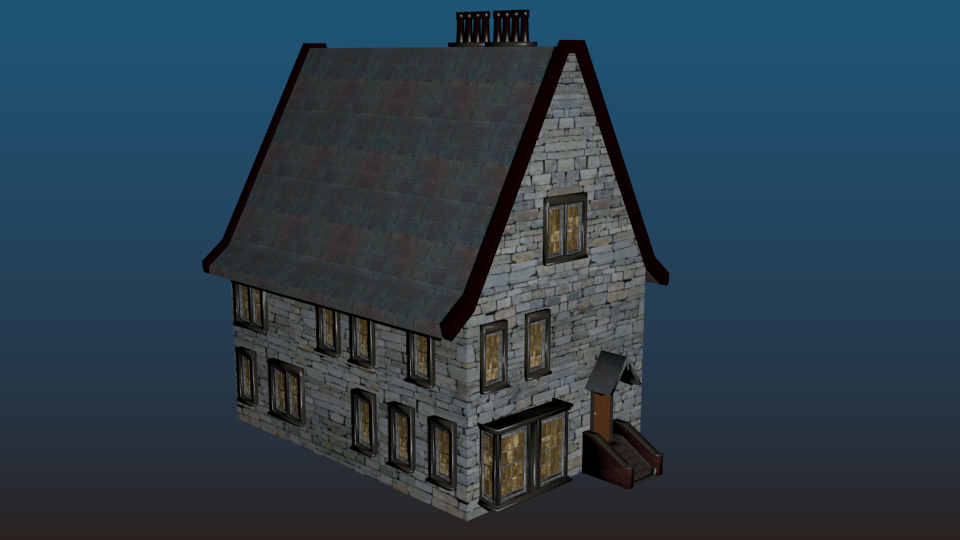
\includegraphics[width=\textwidth]{images/Technique/modelisationMaison.png}
	\caption{\label{fig:modelisationMaison}Une maison réalisée dans Blender}
\end{figure}

Voilà les éléments qui ont été nécessaires pour modéliser la maison qu'on peut voir à la figure \ref{fig:modelisationMaison}:
\begin{itemize}
	\item Le toit: Modélisé à la main; la texture qui permet de simuler les tuiles vient de la 3D Warehouse.
	\item La bordure du toit: Modélisée à la main; cet objet n'a pas de texture mais un seulement un matériau\footnote{Un matériau est un moyen de donner de la couleur à un objet. À l'inverse des textures qui sont des images souvent complexes, les matériaux sont des couleurs unies. On en configure certaines caractéristiques: réflexion, transparence, diffraction de la lumière, etc.} réalisé dans Blender.
	\item Mur de la maison: La géométrie a été réalisée à la main. La texture de mur en pierre provient d'Internet.
	\item La porte: Modélisée à la main, c'est en fait un amalgame de trois objets: le cadre de la porte, la porte et la poignée de la porte. Chacune des parties a son propre matériau.
	\item Les fenêtres simples (9x), doubles (3x) et doubles proéminentes, les cheminées (2x), l'avant-toit et les escaliers proviennent de la 3D Warehouse. Les géométries ont été simplifiées dans Blender; les textures viennent de la 3D Warehouse et d'Internet; elles ont majoritairement été refaites avec Gimp (augmentation des contrastes, assombrissement). Chacun de ces objets est constitué de plusieurs sous-objets eux-mêmes texturés.
\end{itemize}

%Deux objets supplémentaires ont été créés pour ajouter des collisions à la maison. L'un des deux s'applique à la maison entière (pour que le joueur ne puisse pas traverser les murs), l'autre à la porte afin que cette dernière puisse être détectée par \anglicisme{raycast} (\textit{cf.} section \ref{sec:collisions}).

En tout, cette maison comporte:
\begin{itemize}
	\item 9'757 sommets
	\item 11'714 faces
\end{itemize}
À titre de comparaison, un cube simple est formé de 8 sommets et 6 faces.

Anecdote \enquote{amusante}, cette maison, trop lourde à traiter, n'a put être intégrée dans le jeu vidéo final... L'ordinateur ne pouvait supporter une telle quantité de calculs sans surchauffer. De fait, presque aucun des objets retravaillés (fenêtres simples, doubles et doubles proéminentes et les cheminées) n'ont pu être réutilisés.



\subsection{Le retour de la 2D: Textures et images}
\begin{center}
	
\includegraphics[width=.2\textwidth]{images/Technique/gimp.png}
	\\\url{www.gimp.org}
\end{center}

Un jeu 3D ne peut pas se passer d'images! Elles donnent vie aux objets en remplissant la fonction de textures\definition (\textit{cf.} section\ref{sec:textures}). Les interfaces du jeu, comme les menus ou le HUD\definition, sont faites exclusivement à partir d'images. Il faut donc un programme de création/édition d'image. Pour cela, j'utiliserai GIMP (\textit{GNU Image Manipulation Program}). C'est un programme open source, activement soutenu par une grande communauté, ayant atteint un stade de maturité avancé et pour lequel une multitude de tutoriels existent.



\subsection{Réalisation des personnages}
\begin{center}
	
\includegraphics[width=.5\textwidth]{images/Technique/makeHuman.png}
	\\\url{www.makehuman.org}
\end{center}

Un des éléments vitaux pour ce jeu est la création des personnages et de leurs animations. Il existe un outil libre permettant de faire cela: MakeHuman. C'est donc ce dernier que j'ai utilisé pour modéliser tous les personnages présents dans le jeu. Les add-ons\definition\ pour Blender MakeWalk et MakeCloth auront respectivement servi à animer et habiller les personnages.



\subsection{Moteur de jeu}
Godot, le moteur de jeu utilisé, est un programme open source et gratuit, distribué sous la licence MIT, une licence parmi les plus permissives. Il présente un avantage notable: sa compatibilité avec Blender. En effet, l'auteur voulait permettre aux utilisateurs du moteur d'utiliser des outils libres du début à la fin. Il est relativement simple à utiliser comparé à d'autres comme UDK ou UE4 (ces programmes sont d'une complexité extrêmement élevée) et le langage de script qu'il utilise est un dérivé de Python dont la syntaxe est très simple et très lisible. La contrepartie d'une telle caractéristique est que l'implémentation de fonctionnalités avancées prend beaucoup de temps et peut présenter des défis majeurs (alors que, dans les moteurs UDK et UE4 par exemple, de nombreux outils sont à disposition).

\begin{center}
	
\includegraphics[width=.5\textwidth]{./images/Technique/godot_icone.png}
	\\[-1mm]\url{www.godotengine.com}
\end{center}

Le moteur est toujours en développement, il n'est donc pas totalement mature, comporte encore des erreurs et toutes les fonctionnalités ne sont pas disponibles. Le projet étant jeune, la communauté supportant ce projet n'est pas aussi importante que ce que l'on pourrait souhaiter et surtout, la documentation n'est pas complètement écrite. Ce dernier point est le plus critique: il implique de devoir tester au hasard les options non-documentées jusqu'à en comprendre le fonctionnement, ce qui est coûteux en temps et en énergie.

\warningInfo{Configuration des axes dans Godot}{Godot définit les axes de la façon suivante:
	\begin{itemize}
		\item $X$: droite, gauche
		\item $Y$: haut, bas
		\item $Z$: devant, derrière
	\end{itemize}
	À peu près tous les moteurs font pareil. La raison est que, ainsi défini, les axes $X$ et $Y$ représentent les mêmes directions en 2 et en 3 dimensions, ce qui permet une plus grande compatibilité.
	
	Cette convention est utilisée implicitement dans le reste du document.}



\section{Quelques bases pour survivre dans l'univers des jeux vidéo}
\warningInfo{Important}{Les bases données dans les sections suivantes sont très importantes pour la compréhension de la suite de ce travail. Elles sont ensuite utilisées implicitement dans la plupart des explications.}


\subsection{Sommets, arêtes et faces}
Les jeux en trois dimensions sont constitués principalement d'objets, appelés \anglicisme{meshes} en anglais. Ces objets sont, pour leur quasi-totalité, formés exclusivement de faces, d'arêtes et de sommets (\anglicisme{mesh} signifie \enquote{maille}, \enquote{réseau} ou encore \enquote{filet}). Les programmes comme Blender sont spécialisés dans l'édition de tels objets (\textit{cf.} section \ref{sec:modelisationContenu3D}). D'autres types d'objets existent; ils peuvent, par exemple, être formés à partir de courbes. Ces derniers, même s'ils sont utilisés dans les films d'animation, sont en général évités dans les jeux vidéo pour des raisons de performance (\textit{cf.} section \ref{sec:highpolyVersLowpoly}).


\subsection{Calcul des coordonnées}
\subsubsection{Référentiels}
\label{sec:referentiels}
\begin{figure}[th!]
	\center
	\begin{tikzpicture}[x={(\xx cm,\xy cm)}, y={(\yx cm,\yy cm)}, z={(\zx cm,\zy cm)}]
	\draw[thick,->] (0,0,0) -- (5,0,0) node[anchor=north east]{$X$};
	\draw[thick,->] (0,0,0) -- (0,5,0) node[anchor=north west]{$Y$};
	\draw[thick,->] (0,0,0) -- (0,0,5) node[anchor=south]{$Z$};
	\draw(0,0,0) node[anchor=east]{coordonnées globales} node[anchor=south west]{$(0,0,0)$};
	
	\draw[thin, red, dashed](3,0,0) -- (3,0,1);
	\draw[thin, red, dashed](0,0,1) -- (3,0,1);
	\draw[thin, red, dashed](3,0,1) -- (3,4,1) node[anchor=south east, black]{coordonnées locales};
	\draw[->](3,4,1) -- (5,4,1)node[anchor=north east]{$X'$};
	\draw[->](3,4,1) -- (3,6,1)node[anchor=north west]{$Y'$};
	\draw[->](3,4,1) -- (3,4,3)node[anchor=south]{$Z'$};
	
	\draw[thin, blue, dashed] (4,4,1) -- (4,4,2);
	\draw[thin, blue, dashed] (3,4,2) -- (4,4,2);
	\draw[thin, blue, dashed] (4,4,2) -- (4,5,2);
	\draw (4,5,2) -- (4,5,3) -- (5,5,3) -- (5,5,2) -- (4,5,2);
	\draw (4,6,2) -- (4,6,3) -- (5,6,3) -- (5,6,2) -- (4,6,2);
	\draw (4,5,2) -- (4,6,2);
	\draw (4,5,3) -- (4,6,3);
	\draw (5,5,2) -- (5,6,2);
	\draw (5,5,3) -- (5,6,3);
	\end{tikzpicture}	
	\caption{\label{fig:systemeDeCoord}Référentiels et systèmes de coordonnées}
\end{figure}


Dès qu'on parle d'univers en 3 dimensions, la notion de référentiels prend une grande importance. Un référentiel est défini par quatre informations: une origine (le point $(0, 0, 0)$) et la direction des trois axes orthonormés $X$, $Y$ et $Z$. Ils permettent de décrire un point dans l'espace grâce à trois coordonnées: $x$, $y$ et $z$, indiquant une distance depuis l'origine de ces mêmes axes (\textit{cf.} figure \ref{fig:systemeDeCoord}).

Dans le \enquote{référentiel global}, aussi nommé \enquote{monde}, on peut définir des \enquote{sous-référentiels} ou \enquote{référentiels locaux}. Pour définir une telle entité, il faut un point qui donnera l'origine locale (renseignée dans le référentiel global) et trois vecteurs qui renseigneront l'orientation et l'échelle des axes $X'$, $Y'$ et $Z'$. Ces vecteurs donneront l'unité de base des axes dans le référentiel global (ils sont d'ailleurs nommés \enquote{vecteurs-unité}). Cette décomposition permet une grande flexibilité; pour modifier la position, l'orientation ou la taille d'un objet dont les coordonnées sont renseignées localement, il suffit de modifier les vecteurs-unité des axes locaux (rotation et dilatation) ou l'origine (translation).

La figure \ref{fig:systemeDeCoord} donne une idée de ce fonctionnement:
\begin{itemize}
	\item Le référentiel local, défini par les axes $X'$, $Y'$ et $Z'$, a son origine au point global $(6, 8, 2)$. Les traits rouges indiquent les coordonnées de cette position.
	\item Les axes $X'$, $Y'$ et $Z'$ sont définis respectivement le long des axes $X$, $Y$ et $Z$. Leur norme --- ou longueur --- équivaut à $1$.
	\item L'objet \enquote{cube} est défini dans le référentiel local. Les coordonnées d'un des points du cube sont données par les traits bleus.
\end{itemize}
Il suffit maintenant de changer l'origine du référentiel local pour que le cube soit translaté ou de modifier les vecteurs-unité des axes $X'$, $Y'$ et $Z'$ pour que ce cube pivote ou change d'échelle.

\textbf{Exemple}\quad Imaginons un instant qu'on fasse pivoter le référentiel local autour de l'axe $Z'$ de 90°. L'axe $Y'$ sera orienté horizontalement vers la gauche et $X'$ pointera vers le haut. Les coordonnées du cube sont données dans le référentiel local, cela implique que, si localement cela ne change rien, dans l'espace global, le cube pivote en même temps que ses axes.

Tous les programmes de modélisation ainsi que les moteurs de jeu utilisent cette méthode: \textit{chaque} objet est défini dans son référentiel local.

\subsubsection{Calcul matriciel}
\label{section:calculMatriciel}
\vspace*{-\baselineskip}
\begin{figure}[ht!]
	\center
	\begin{tikzpicture}[x={(\xx cm,\xy cm)},y={(\yx cm,\yy cm)},z={(\zx cm,\zy cm)},]
		% rectangle ecran
		\draw (-2,1,-5) -- (-2,-1,-5) -- (2,-1,-5) -- (2,1,-5) -- (-2,1,-5);
		%traits point de vue ecran
		\draw (0,0,0) -- (-2,1,-5);
		\draw (0,0,0) -- (-2,-1,-5);
		\draw (0,0,0) -- (2,1,-5);
		\draw (0,0,0) -- (2,-1,-5);
		%traits tilles
		\draw [dashed] (-2,1,-5) -- (-3,1.5,-7.5);
		\draw [dashed] (-2,-1,-5) -- (-3,-1.5,-7.5);
		\draw [dashed] (2,1,-5) -- (3,1.5,-7.5);
		\draw [dashed] (2,-1,-5) -- (3,-1.5,-7.5);
		%texte
		\draw (0,0,0) node [below] {point de vue};
		\draw (0,1,-5) node[above] {écran};
		%cube
		\draw (0,0,-12) -- (0,1,-12) -- (1,1,-12) -- (1,0,-12) -- (0,0,-12);
		\draw (1,0,-12) -- (1,0,-13);
		\draw (0,1,-12) -- (0,1,-13);
		\draw (1,1,-12) -- (1,1,-13);
		\draw (1,0,-13) -- (1,1,-13) -- (0,1,-13);
		\draw (0,0,-12) node[below, left]{monde 3D};
	\end{tikzpicture}
	\caption{Projection du monde 3D sur un écran\label{fig:projectionMonde3D}}
\end{figure}

L'ordinateur dispose maintenant d'un univers en 3 dimensions dans lequel se trouvent les objets du jeu. Mais cela ne permet pas d'obtenir une image à l'écran; la machine doit encore convertir l'environnement 3D en une image 2D. Pour cela, deux opérations sont nécessaires. Premièrement, toutes les coordonnées doivent être obtenues dans le référentiel global, on parle ici de changement de référentiel. Deuxièmement, il faut choisir un point de vue puis projeter sur un écran ce qu'on peut voir du monde depuis ce point de vue. Cela revient à projeter tous les objets 3D en 2D, en tenant compte des parties cachées. Godot se charge seul de ces deux opérations qui sont effectuées à l'aide de matrices. Voir la figure \ref{fig:projectionMonde3D} pour une illustration du processus de projection.

Cependant, toutes les modifications que l'informaticien voudrait apporter à un objet depuis le code doivent être apportées au moyen d'une multiplication matricielle. Les transformations géométriques sont donc un élément important à comprendre. Par exemple, toutes les translations, rotations ou encore tous les changements d'échelle décrits plus haut sont appliqués en utilisant du calcul vectoriel ou matriciel. De telles notions n'étant pas enseignées à notre niveau, j'ai dû compléter mes connaissances mathématiques.



\subsection{Normales}
\label{sec:normales}
Les normales sont des vecteurs utilisés pour décrire l'orientation d'une face dans l'espace. Elles permettent de savoir sur quel plan se situe une face. Ce sont des vecteurs normalisés (de longueur $1$), perpendiculaires en tout point à la face. Dans les moteurs graphiques comme Godot, elles indiquent aussi dans quelle direction pointe la face (elle a un \enquote{haut} et un \enquote{bas}).


\newpage
\subsection{Introduction à GDScript}
\criticalInfoDarkRed{Confusion sur le sens du mot \enquote{objet}}{Le mot \enquote{objet} peut prendre deux sens extrêmement distincts selon le contexte dans lequel il est utilisé. Lorsqu'on parle de modélisation, un objet représente une forme en trois dimensions avec des textures, qui est intégrée dans le jeu. En programmation, il désigne un concept fondamental des langages informatiques modernes: une structure qui peut contenir des fonctions et des variables. La programmation orientée objet est un élément vital dans les logiciels modernes et les jeux vidéos ne font pas exception à cette règle.}

GDScript est le langage utilisé dans Godot. Sa syntaxe est très proche de Python et très lisible. Voilà les quelques bases à connaître pour pouvoir comprendre les extraits de code présentés ici.\cite{godotenginegodot_}

Le mot-clé \lstinline|var| sert à déclarer une variable, à savoir une entité qui peut contenir n'importe quel type d'objet: un entier, un nombre à virgule, un tableau, un dictionnaire\footnote{En programmation, un dictionnaire est un tableau particulier qui fait correspondre des clés (souvent des chaines de caractères) à des valeurs (tout comme un dictionnaire fait correspondre un mot à une définition).}, etc.

Le mot-clé \lstinline|func| permet de définir une fonction. Il est immédiatement suivi par le nom de la fonction définie ainsi que d'une paire de parenthèses qui peut éventuellement contenir des arguments.

Tout ce qui suit un \lstinline|#| et qui est sur la même ligne est un commentaire. En programmation, cette notion désigne du texte qui n'est pas considéré comme du code et est ainsi ignoré par l'ordinateur. Ces caractères sont destinés uniquement aux utilisateurs qui liront le programme afin de faciliter la compréhension du code. Tous les codes présentés dans ce texte sont largement commentés.

Le langage GDScript utilise le niveau d'indentation pour délimiter les blocs logiques. Le nombre de \enquote{tabulations\footnote{La touche nommée \enquote{tab} sur le clavier permet d'ajouter des caractères de tabulation. Ces derniers ajoutent un espace blanc plus grand que l'espace habituel (souvent équivalent à 3 espaces)}} au début d'une ligne donne son niveau d'indentation. Un bloc logique est composé de lignes à la suite les unes des autres et possédant le même niveau d'indentation, et éventuellement de sous-blocs logiques.


\renewcommand{\codeTitle}{Les bases de GDScript}
\begin{lstlisting}[caption=basics.gd]
var nombreDeGardes = 4 #déclaration d'une variable
nombreDeGardes = plusDeux(nombreDeGardes) #appel d'une fonction avec la variable nombreDeGardes passée en paramètre

func maFonction(): #cette ligne déclare une nouvelle fonction nommée maFonction
	var variable1 = 7 #nouvelle variable dont la valeur est 7
	variable2 = ['un', 'deux', 'trois'] #variable assignée à un tableau contenant trois chaines de caractères

func plusDeux(argument1):
	return argument1 + 2
\end{lstlisting}

% #On constate bien que le niveau d'indentation à une signification importante: les lignes 1 et 2 sont du code normal exécuté immédiatement; les lignes 5 et 6 appartiennent à la ligne 4 et forment un groupe logique qui définit une fonction.



\section{Techniques utilisées dans {\fontspec{Great Vibes}Eluria's Chronicles}}
\subsection{Textures}
\label{sec:textures}
Les textures sont des images appliquées sur un objet pour lui donner de la couleur, ajouter des détails à la géométrie (\textit{cf.} section \ref{sec:highpolyVersLowpoly} sur les \anglicisme{normal map} et  \anglicisme{bump map}), modifier la quantité ou la couleur des reflets, définir les zones qui émettent de la lumière et leur couleur (\anglicisme{glow map}), etc. Elles sont très largement utilisées dans les jeux vidéos ainsi que les films d'animation car peu coûteuses en matière de calcul.

Pour appliquer une image en 2 dimensions sur un objet en 3 dimensions, la technique la plus souvent utilisée est appelé \anglicisme{UV unwrapping}\footnote{UV fait référence aux axes U et V de la texture. En effet, pour ne pas confondre les coordonnées de la texture avec d'autres, les axes ont été nommés différemment. Attention à ne pas confondre UV avec Ultra-Violets.}. L'idée est de \enquote{découper} un objet afin de le déplier et de le poser \enquote{à plat} (\textit{cf.} figure \ref{fig:uvUnwrap}). Une fois cette opération effectuée, il devient simple d'appliquer la texture sur l'objet. Cette méthode a cependant le désavantage de distordre les textures une fois appliquées aux faces d'objets compliqués.

\begin{figure}[th!]
	\center
	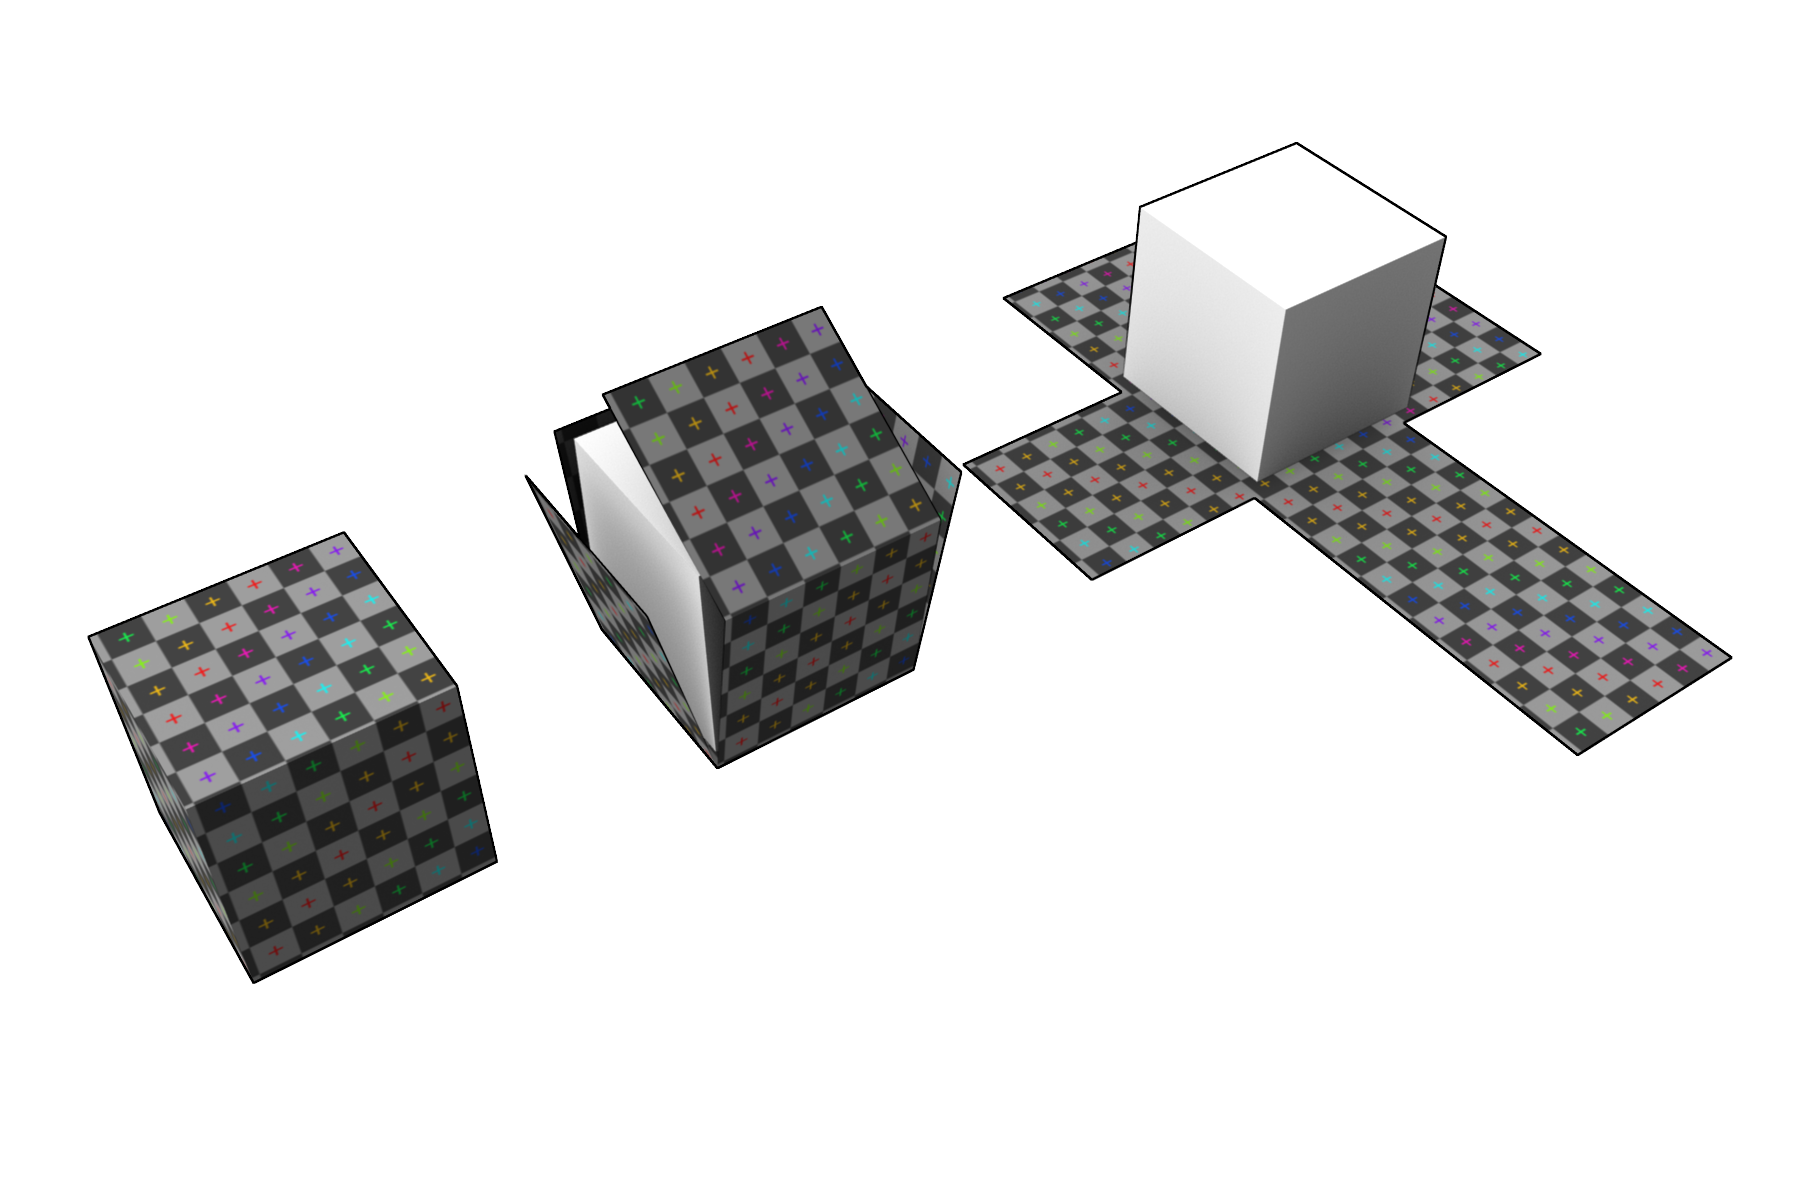
\includegraphics[width=.5\textwidth]{images/Technique/uvUnwrap.png}
	\caption{\label{fig:uvUnwrap}UV Unwrapping d'un cube {\cite{CubeRepresentativeUVUnwrapping_}}}
\end{figure}

Dans \nomJeu, tous les objets dont la couleur n'est pas simplement unie utilisent une texture de couleur. De même, les objets qui émettent de la lumière comme les enseignes lumineuses utilisent des \enquote{textures de rougeoiement} (\anglicisme{glow texture}). Les images sont créées dans GIMP, appliquées dans Blender par \anglicisme{UV unwrapping} et finalement exportées dans le moteur de jeu pour le rendu final.



\subsection{Highpoly vers Lowpoly}
\label{sec:highpolyVersLowpoly}
Le temps de calcul par image est un aspect très important lors de la réalisation d'un jeu vidéo. Trop élevé, il empêchera l'ordinateur d'afficher suffisamment d'images à la seconde pour rendre le flux vidéo fluide. Parmi les facteurs qui influent sur cette valeur critique, on notera principalement le nombre de sommets et de faces dans la scène. En effet, il faut calculer pour chaque face la position à l'écran des sommets (\textit{cf.} section \ref{section:calculMatriciel}), la quantité de couleur émise, les reflets, le z-index ou indice de profondeur\footnote{Le z-index décrit quelle est la face la plus proche de la caméra afin de n'afficher que cette dernière. Sans lui, ce serait la dernière face calculée qui serait affichée...}, etc.

Les objets utilisés doivent donc être les plus économes possible en matière de géométrie. Une technique très couramment utilisée pour diminuer le nombre de sommets avec un minimum de perte de qualité est celle du \anglicisme{normal mapping}.

On commence par réaliser un modèle très simplifié de l'objet. Ce dernier ne fera que rarement plus de 500 faces dans le cas d'un objet non-animé --- c'est le Lowpoly (\anglicisme{low}, bas ou peu; et \anglicisme{poly} pour polygone). On le duplique ensuite pour ajouter à la copie tous les détails désirés. Ce deuxième modèle peut posséder des millions de faces. Une fois cette opération terminée, on \enquote{cuit} (traduction littérale du terme anglais \anglicisme{bake} qui désigne cette manipulation) les différences de hauteur entre les deux objets sur une texture (\textit{cf.} section \ref{sec:textures}). Autrement dit, les différences de hauteur se trouvent renseignées sur une image 2D, codées en couleurs.

Il est possible de générer plusieurs types de texture: des \anglicisme{normal map} (pas vraiment de traduction) ou des \anglicisme{bump map} (\enquote{placage de relief} en français). Les premières sont codées en trois couleurs --- Rouge, Vert, Bleu --- soit trois informations qui représentent les translations sur les axes $X$, $Y$ et $Z$ de chaque point. La deuxième, plus simple, est une image en niveau de gris, soit à une seule dimension (le degré de noirceur) qui déterminera la translation de chaque point le long de la normale (\textit{cf.} section \ref{sec:normales}) de la face.

Ces textures sont appliquées sur l'objet Lowpoly. L'ordinateur calcule ensuite les ombres et certains détails comme si les sommets s'étaient réellement déplacés, donnant l'impression d'un niveau de détail très élevé bien que la géométrie de l'objet n'ait pas changé. Ceci permet, sans trop de perte de qualité, de faire passer le nombre de sommets par objet de plusieurs millions à quelques centaines seulement. Cette technique est très utilisée et on la retrouve dans tous les jeux vidéos modernes. Voir la figure \ref{fig:normalMapping} pour une illustration graphique du processus.

\begin{figure}[th!]
	\center
	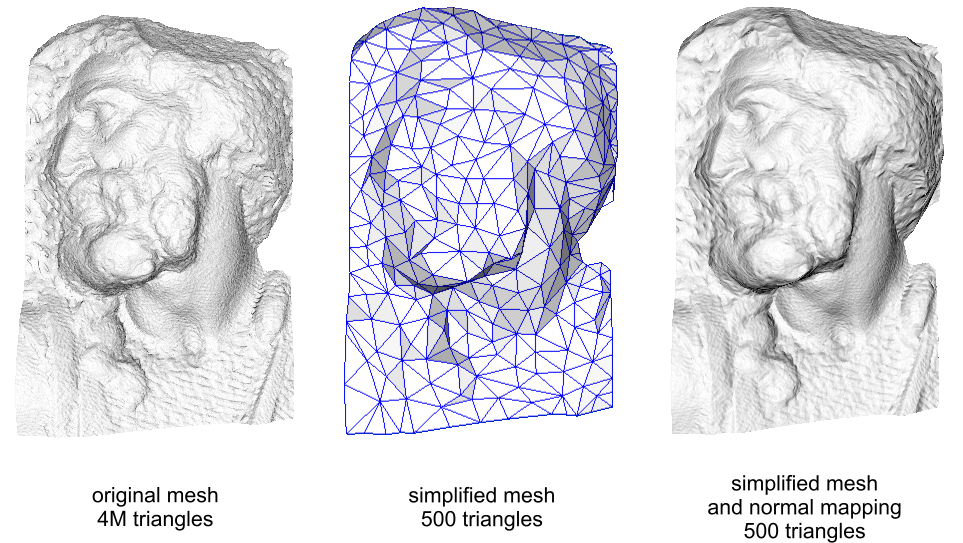
\includegraphics[width=.8\textwidth]{images/Technique/Normal_map_example.png}
	\caption{Exemple de \anglicisme{normal mapping\label{fig:normalMapping}} {\cite{Normalmappingusedtoredetailsimplifiedmeshes_}}}
\end{figure}


\subsection{Collision et \anglicisme{Raycast}}
\label{sec:collisions}
Si nous avons tous une perception intuitive des collisions avec la matière et de leurs effets dans la réalité, l'ordinateur n'a pas cette connaissance. Pour que l'univers virtuel devienne tangible, solide, il faut que l'ordinateur calcule les chocs et les conséquences qu'ils ont dans le jeu. Il faut donc ajouter pour chaque objet des \enquote{collisions}, soit une géométrie supplémentaire qui exécute du code lorsqu'un autre objet vient à la chevaucher. Il existe différents types de réponses possibles: l'objet peut ne pas bouger du tout, ricocher, faire ricocher l'autre, etc.

Une grande partie de ces calculs compliqués est prise en charge par le moteur physique de Godot. Il peut s'occuper de certains comportements par défaut comme les objets statiques ou ceux effectuant des mouvements simples. Mais les collisions d'un joueur, par exemple, sont nettement plus complexes à gérer: il faut qu'il puisse sauter, ce qui implique de la gravité (ajoutée par programmation); s'il y a des combats dans le jeu, le joueur doit pouvoir être touché et les dégâts éventuellement calculés en fonction du lieu d'impact, etc. Tout cela doit être codé à la main.

Le \anglicisme{Raycast} également nécessite des collisions pour pouvoir fonctionner. Cette technique permet de tirer un rayon\footnote{Aucun rayon n'est jamais tiré, c'est simplement une métaphore qui représente, dans la réalité, des calculs mathématiques.} depuis un objet ou l'écran et de voir quelle est la première géométrie de collision rencontrée. Cela permet de déterminer beaucoup de choses utiles: quel objet se trouve sous le curseur du joueur, l'ennemi peut-il détecter le joueur ou un mur bloque-t-il son champ de vision, etc.



\section{Code d'exemple --- Gestion de la caméra}

Dans un jeu vidéo à la première personne\footnote{Un jeu vidéo à la première personne est un jeu vidéo dans lequel le joueur est  le héros et voit par ses yeux. À l'inverse, dans un jeu vidéo à la troisième personne, le joueur voit le personnage qu'il contrôle; il est à l'extérieur du corps du personnage.}, l'orientation de la caméra est toujours gérée par l'utilisateur. Pour les jeux d'ordinateur, la souris est généralement affectée à cette tâche.

Il faut donc convertir les mouvements de la souris (translations 2D) en mouvements de caméra (rotations 3D). Les coordonnées $x$ de la souris détermineront les rotations horizontales (autour de l'axe $Y$) et les coordonnées $y$, celles verticales (autour de l'axe $X$). Toutes ces opérations doivent se faire sur le référentiel local de la caméra. Une implémentation simple est de coupler les déplacements de la souris sur les axes $X$ et $Y$ avec une rotation de la caméra autour des axes $Y$ et $X$:
\begin{align*}
		\delta x \cdot \kappa &= rotation_Y\\
		\delta y \cdot \kappa &= rotation_X
\end{align*}

Avec $\kappa$, le coefficient qui contrôle la vitesse de rotation de la caméra, et $\delta x$ et $\delta y$, les mouvements de la souris (considérés comme des angles en radians).

Cette implémentation est cependant incorrecte. On peut le voir avec l'exemple suivant:
\begin{enumerate}
	\item On fait une rotation verticale (selon l'axe local $X$) pour que la caméra regarde vers le haut avec un angle de 45°
	\item On fait pivoter la caméra horizontalement (selon l'axe local $Y$)
\end{enumerate}

L'étape numéro 2 va poser problème. En effet l'axe vertical local ($Y$) de la caméra a pivoté lors de l'étape 1 et fait un angle de 45°. Une rotation autour de cet axe aura pour conséquence de faire tourner la caméra \enquote{de biais}, donnant l'impression que la caméra tombe de son pivot. Un tel effet n'est évidemment pas désiré.

Il faut donc trouver une autre formule pour convertir les mouvements de la souris en rotation de caméra. Une bonne méthode consiste à les coupler aux angles polaires $\theta$ et $\varphi$ puis à utiliser la formule de conversion entre coordonnées sphériques et cartésiennes\cite{Coordonneesspheriques_}.

Les coordonnées sphériques servent à représenter des points dans l'espace (\textit{cf.} figure \ref{fig:coordonneesSpheriques}). Elles sont très souvent utilisées en cartographie. Les trois coordonnées sont données par:
\begin{itemize}
	\item Le rayon $\rho$ de la sphère sur laquelle se situe le point $P$ (soit la distance origine--point).
	\item Un angle horizontal, compris entre 0 et 2$\pi$, noté $\theta$
	\item Un angle vertical, compris entre 0 et $\pi$, noté $\varphi$
\end{itemize}
Ces coordonnées fonctionnent donc à l'aide de deux angles, exactement ce que les mouvements de la souris fournissent.

\begin{figure}[th!]
	\center
	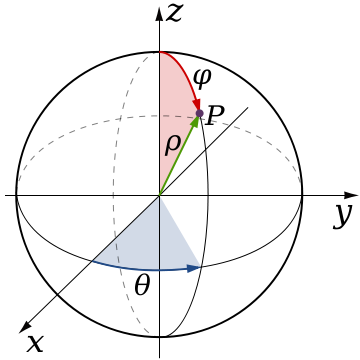
\includegraphics[width=5cm]{images/Technique/coordonneesSpheriques.png}
	\caption{\label{fig:coordonneesSpheriques}Coordonnées sphériques{\cite{Adiagramofsphericalcoordinatesdefiningapointbycolatitudelongitudeandradius_Wikipedia}}}
\end{figure}

Les coordonnées cartésiennes sont celles dont nous avons l'habitude, avec trois composantes: $x$, $y$ et $z$. La formule de conversion entre les deux systèmes est la suivante:
\begin{equation}
	\left\{
	\begin{array}{ll}
		x &= \rho \cos \theta\\
		y &= \rho \sin \theta \cos \varphi\\
		z &= \rho \sin \theta \sin \varphi
	\end{array}	
	\right.
	\label{eqn:coordonneesSpheriquesVersCartesiennes}
\end{equation}
Nous pouvons maintenant transformer les mouvements de la souris sur les axes $X$ et $Y$, en les couplant respectivement à $\theta$ et $\varphi$. Mais comment faire pivoter la caméra de la bonne façon avec de telles données?

Godot fournit une fonction --- \lstinline{Transform.looking_at(Vector3 point, Vector3 haut)} --- qui s'applique à un objet de type \lstinline{Transform} (qui représente un référentiel, \textit{cf.} section \ref{sec:referentiels}) et retourne une copie de ce référentiel mais pivoté de manière à ce qu'il regarde en direction de \lstinline{point}. Il ne reste plus qu'à calculer les coordonnées de \lstinline{point}. Pour ce faire, il faut ajouter aux coordonnées globales de la caméra le vecteur normalisé obtenu grâce à la formule \ref{eqn:coordonneesSpheriquesVersCartesiennes}. \lstinline{Point} se trouvera ainsi toujours dans une sphère de rayon 1 autour de la caméra qui le \enquote{suivra des yeux}.

\normalInfo{\lstinline{get_transform} et \lstinline{set_transform}}{Les méthodes \lstinline{get_transform} et \lstinline{set_transform} permettent respectivement d'obtenir et de définir le système de coordonnées locales d'un objet (orientation et position). C'est donc ces dernières qui sont utilisées pour faire pivoter la caméra.}

\renewcommand{\codeTitle}{Code de la caméra}
\begin{lstlisting}[caption=cameraControls.gd]
var view_sensitivity = 0.1
var angleHorizontal = 0 #angle horizontal de départ
var angleVertical = 90 #angle vertical de départ (droit devant)

func _ready(): #exécuté une fois au début
	set_transform(get_transform().looking_at(Vector3(0, 0, 1) + get_transform().origin, Vector3(0, 1, 0))) # définit le premier angle de la camera	
	
	Input.set_mouse_mode(2) #souris invisible, fixée au centre
	set_process_input(true) #la fonction _input sera exécutée à chaque fois que la caméra reçoit des inputs (dont les mouvements de souris)

func _input(ev): #cette fonction est exécutée à chaque fois que la souris bouge et gère la rotation de la caméra en fonction des mouvements de la souris
	if ev.type==InputEvent.MOUSE_MOTION:
		angleHorizontal = fmod(angleHorizontal + ev.relative_x * view_sensitivity, 360) #cette ligne ajoute à angleHorizontal le déplacement de la souris sur l'axe x multiplié par la sensibilité de la caméra puis retourne le reste de la division entière de angleHorizontal par 360 afin que cette variable ait toujours une valeur entre 0 et 360
		angleVertical = angleVertical + ev.relative_y * view_sensitivity #on ajoute à angleVertical le déplacement de la souris sur l'axe y multiplié par la sensibilité de la caméra
		
		#les quatre lignes suivantes empêchent angleVertical d'avoir une valeur supérieure à 180 ou inférieure à 0
		if angleVertical>180:
			angleVertical = 180
		if angleVertical<0:
			angleVertical = 0
		
		set_transform(get_transform().looking_at(where_to_look_at(angleHorizontal, angleVertical) + get_transform().origin, Vector3(0, 1, 0))) #cette ligne est très importante, elle change l'orientation de la caméra pour qu'elle pointe vers le point obtenu en ajoutant l'origine de la caméra au résultat de where_to_look_at

func where_to_look_at(theta_degré, phi_degré):
	var theta = deg2rad(theta_degré)
	var phi = deg2rad(phi_degré)
	var sin_theta = sin(theta)
	var sin_phi = sin(phi)
	
	return Vector3(sin_theta*sin_phi, cos(theta), -1 * sin_theta * cos(phi))
#c'est cette fonction qui fait la conversion entre coordonnées sphériques et cartésiennes C'est le coeur de l'algorithme. On remarquera d'ailleurs que la formule utilisée est la même que celle décrite juste au dessus
# (phi: 0°=regarde droit devant, positif a droite, negatif a gauche)
# (theta: 90°=regarde à l'horizontale, 0°=regarde en haut, 180=regarde en bas)
# Les angles doivent être compris entre -360 et 360 pour horizontal, entre 0 et 180 pour vertical
\end{lstlisting}


\section{Quelques problèmes rencontrés}

\begin{note}
	Cette section détaille quelques problèmes sur lesquels je suis tombé et donne des informations utiles pour mieux envisager le travail dans sa globalité. Elle ne se veut pas une liste exhaustive de tous les problèmes rencontrés, ce serait trop long.
\end{note}

\subsection{Les normales, de Sketchup à Blender}
La normale d'une face pointe normalement vers l'extérieure de cette dernière. Ainsi, un objet dont les normales seraient visibles ressemblerait à un hérisson (toutes les normales pointant vers l'extérieur de l'objet).

Afin de réaliser le moins de calculs possible, certains moteurs de jeu n'affichent que les faces qui pointent vers la caméra; à savoir, uniquement les faces dont la normale est orientée dans sa direction. Ceci permet, théoriquement, de diviser par deux le nombre de faces dont il faut faire le rendu et ainsi le temps de calcul pour une image. Bien que les cartes graphiques qui font ces calculs soient de plus en plus puissantes, beaucoup de moteurs de jeu utilisent ce procédé.

Godot n'est pas une exception. Il est également possible d'afficher toutes les faces, quelles que soient leur direction, mais cela n'est pas recommandé. En effet, pour que le jeu reste fluide, il faut au minimum 24 images par seconde (ou fps pour \anglicisme{Frame Per Second}) mais 60 est la norme recommandée pour que le joueur ne soit jamais dérangé par des images \enquote{sautantes}.

Cette spécificité des jeux vidéos ne pose généralement pas de problème. Par exemple, dans le cas d'objets modélisés dans Blender, étant donné que tout s'y fait à partir de formes primitives (cubes, cylindres, etc.) dont les faces sont bien orientées, la transition vers un moteur de jeu se fait sans problème. Mais prenons maintenant le cas d'objets importés de la 3D Warehouse de Google (\textit{cf.} section \ref{sec:modelisationContenu3D}) puis convertis pour Blender. Le programme utilisé par défaut pour le visionnement et l'édition des fichiers de la librairie en ligne, Google SketchUp, n'est pas (ou peu) sensible à l'orientation des faces. Ainsi, certains modèles arrivent dans Blender avec une partie de leurs normales mal orientées... Mais Blender n'est pas touché par ce problème: tout comme Google SketchUp, il affiche toutes les faces, quelle que soit leur disposition. C'est au moment de passer l'objet dans le moteur de jeu que la moitié des faces disparaissent, car ce programme, lui,  est sensible à la direction des normales!

Un objet, dans cet état, est inutilisable dans le moteur de jeu. Deux solutions s'offrent alors: inverser à la main ou de façon semi-automatisée les faces dans Blender, ce qui représente un travail long et fastidieux. Ou alors, changer carrément d'objet, par exemple en le modélisant à la main. Heureusement, tous les fichiers ne présentent pas ce genre de difficultés. Mais ceux qui en souffrent  sont souvent irrécupérables et font perdre un temps précieux. De plus, ce problème, lorsqu'il est rencontré pour la première fois surprend beaucoup (et peut causer un certain énervement).


\subsection{Importation des textures dans Godot}
Blender dispose d'une interface très puissante pour créer des matériaux. Il est possible d'en inventer une grande quantité, pouvant ressembler à n'importe quelle matière réelle. Le nombre d'options configurables est tout simplement affolant. Pas étonnant que les matériaux soient une des difficultés majeures de ce programme qui effraie encore et toujours les novices (moi compris).

Godot est écrit de façon à être compatible avec Blender. Cependant, n'ayant pas encore atteint un niveau élevé de maturité, nombreux sont encore les bugs concernant l'importation de textures. De fait, ces dernières devraient normalement être créées directement dans le moteur de jeu pour éviter tout problème. Il est cependant impossible de remplir une telle exigence dès que l'on désire utiliser des textures de couleurs ou des normales map (par opposition aux \enquote{textures procédurales}), l'\anglicisme{UV unwrapping} devant se faire avec Blender. De plus, la plupart des objets provenant de la 3D Warehouse sont déjà texturés. N'oublions pas non plus que les multiples conversions de format entre Google Sketchup et Blender puis entre Blender et Godot ne facilitent pas la transition.

À de multiples reprises, les objets sont arrivés gris (couleur par défaut $\rightarrow$ texture non importée) dans le moteur de jeu. Il m'aura fallu beaucoup de temps pour comprendre la source du problème (pour être plus exact, \textit{les} sources du problème).

Utilisant de multiples répétitions du même objet dans Blender, j'ai créé des références vers ces objets dans mes scènes, plutôt que de copier chaque objet dont j'avais besoin. De cette façon, si je modifiais l'objet, il changeait également dans toutes les scènes où il était référencé. C'est une façon de dire à Blender \enquote{Mets l'objet \textit{x} à cet endroit dans la scène. Pour trouver les données de cet objet, ouvre le fichier \textit{xxx.blend}.} Si l'idée paraissait excellente, il s'est avéré que l'exporteur ne supporte pas cette option et retourne une erreur relative aux textures.

Ce premier problème me causa beaucoup de soucis conjointement avec un autre. En effet, une fois la question de l'importateur réglée et l'objet importé, les textures apparaissaient grises. Elles n'avaient donc pas été importées. Cela provenait du fait que Godot stocke dans le cache (garde en mémoire) les textures qu'il a déjà copié à l'importation précédente. Modifier ces textures, à moins de réimporter l'objet complètement, n'a donc pas d'effet dans le moteur de jeu.

La combinaison déroutante de ces deux bugs me coûta plusieurs heures avant d'être résolu correctement (enfin je crois... J'ai, de fait, toujours des problèmes avec cette importation).

\subsection{Animation des personnages}
Modéliser un humain représente un véritable casse-tête. La complexité du corps est telle qu'il est impossible d'obtenir un résultat satisfaisant sans passer des jours derrière l'écran. Ainsi, j'ai décidé d'utiliser MakeHuman, un logiciel libre et gratuit, pour créer mes personnages. Ce programme propose une interface très complète pour créer des êtres humains de toutes sortes, toutes les couleurs de peau, toutes les corpulences, etc. Un modèle spécial jeu vidéo est proposé, contenant beaucoup moins de sommets afin de soulager le processeur d'une surcharge de calculs. Enfin l'importation dans Blender est quasiment transparente et pose généralement peu de difficultés.

Celles-ci se présentent au moment d'animer le personnage. Les techniques d'animation modernes requièrent un studio, des acteurs, des caméras 3D et une grosse puissance de calcul (les mouvements des acteurs sont immédiatement appliqués aux personnages en 3 dimensions). Cette technique était bien sûr exclue d'office pour moi. Autre possibilité, tout modéliser à la main. Mais, une fois de plus, l'univers de l'animation est très particulier et pour arriver à un résultat convaincant, des centaines d'heures sont probablement nécessaires. Une cinématique \enquote{aussi simple} que la marche est très difficile à modéliser pour paraître réaliste et fluide.

La solution était donc de trouver sur internet des fichiers contenant déjà la digitalisation d'animations capturées avec les méthodes professionnelles. Et de tels fichiers existent. Ils sont même relativement répandus.

Mais les vrais ennuis arrivent au moment d'appliquer ces animations aux personnages. Les fichiers contiennent les modifications à appliquer à chaque os de l'armature contrôlant la géométrie du personnage\footnote{Les géométries compliquées, pour simplifier leur animation, sont contrôlées grâce à des \enquote{os}. Ce sont des entités auxquelles sont attribués certains sommets de la géométrie de l'objet. Ainsi en faisant bouger un os, tous les sommets qui lui sont liés bougent simultanément.} sur chacun des axes à chaque image. On voit immédiatement les multiples complications qui peuvent apparaître: comment faire si le nombre d'images par seconde dans le fichier n'est pas le même que dans Blender? Les animations se dérouleront au ralenti ou en accéléré. Et que faire si l'armature utilisée dans le fichier d'animation n'est pas la même que celle de l'objet à animer?

Pour cela, l'addon MakeWalk de Blender est simplement impressionnant. Il est capable de modifier la vitesse de l'animation seul, mais mieux encore, il est capable de comprendre quels os de l'animation représentent quels os du personnage! Cependant, un processus d'une telle complexité ne peut toujours réussir. Ainsi il n'est pas rare d'avoir des problèmes mineurs mais cependant dérangeants dans les animations. Par exemple, l'animation \enquote{marcher}, une fois appliquée, causait aux personnages d'avoir les chevilles et les pieds étrangement orientés vers l'intérieur.

Il a donc fallu jouer avec les options de configuration de MakeWalk, comprendre les possibilités qu'il offre, etc.